\section{Simulation Analysis}
\label{sec:simulation}

In this section, Ngspice was used in order to simulate the Audio Converter. A brief description of the circuit modeled in NGspice is going to be presented and a comparison between the values obtained in NGspice and the ones in Octave is going to be done as well. In order to do that, transistors of the given models were used and the rest of the components specifications changed to be on par with the values through MatLab.

In the next sections we are interested in the two impedances associated with the circuit as a whole ($Z_{in}$ and $Z_{out}$), both cut-off frequencies ($f_{CO_L}$ and $f_{CO_H}$), the bandwidth (interval between the cut-off frequencies) and the total gain measured in the bandpass region. The measurement of these parameters and the overall performance of the circuit is well represented in the section \ref{merit}.\par 

Besides that, we also confirmed whether the BJTs are on the Forward Active Region (FAR), by comparing $V_{CE}$ and $V_{BE}$ for the NPN (and, similarly, $V_{EC}$ and $V_{EB}$ for PNP).
The confirmation is presented below, to the NPN and PNP respectively:

\begin{table}[H] \centering
\begin{tabular}{|
>{\columncolor[HTML]{FFCC67}}l |c|}
\hline
\multicolumn{2}{|l|}{\cellcolor[HTML]{EABD8B}Name - Value} \\ \hline
V_CE&4.71217\\ \hline
V_BE&0.642988\\ \hline
V_CE>V_BE & Correct F.A.R\\ \hline

\end{tabular}
\caption{NPN Voltages and FAR confirmation}
\end{table}

\begin{table}[H] \centering
\begin{tabular}{|
>{\columncolor[HTML]{FFCC67}}l |c|}
\hline
\multicolumn{2}{|l|}{\cellcolor[HTML]{EABD8B}Name - Value} \\ \hline
V_CE&6.83806\\ \hline
V_EB&0.785099\\ \hline
V_EC>V_EB & Correct F.A.R\\ \hline

\end{tabular}
\caption{PNP Voltages and FAR confirmation}
\end{table}

The following table represents the results obtained from simulation in NGSpice:

\begin{table}[H] \centering
\begin{tabular}{|
>{\columncolor[HTML]{FFCC67}}l |c|}
\hline
\multicolumn{2}{|l|}{\cellcolor[HTML]{EABD8B}Name - Value} \\ \hline
V-Gain & 34.1988\\ \hline
Bandwidth & 1.22501E+06\\ \hline
CO-lowerFreq & 15.8734\\ \hline
CO-higherFreq & 1.22503E+06\\ \hline

\end{tabular}
\caption{Results for the output}
\end{table}

\subsection{Coupling Capacitor}

In our Amplifier circuit there are two coupling capacitors ($C_{in}$ and $C_O$) but, since their functions are equivalent, we will focus on the first capacitor, the $C_{in}$ . \par 
Below, is shown the frequency response analysis to the different values of C, changing the parameter drastically.

\begin{figure}[H] 
\centering
\begin{subfigure}{0.4\textwidth}
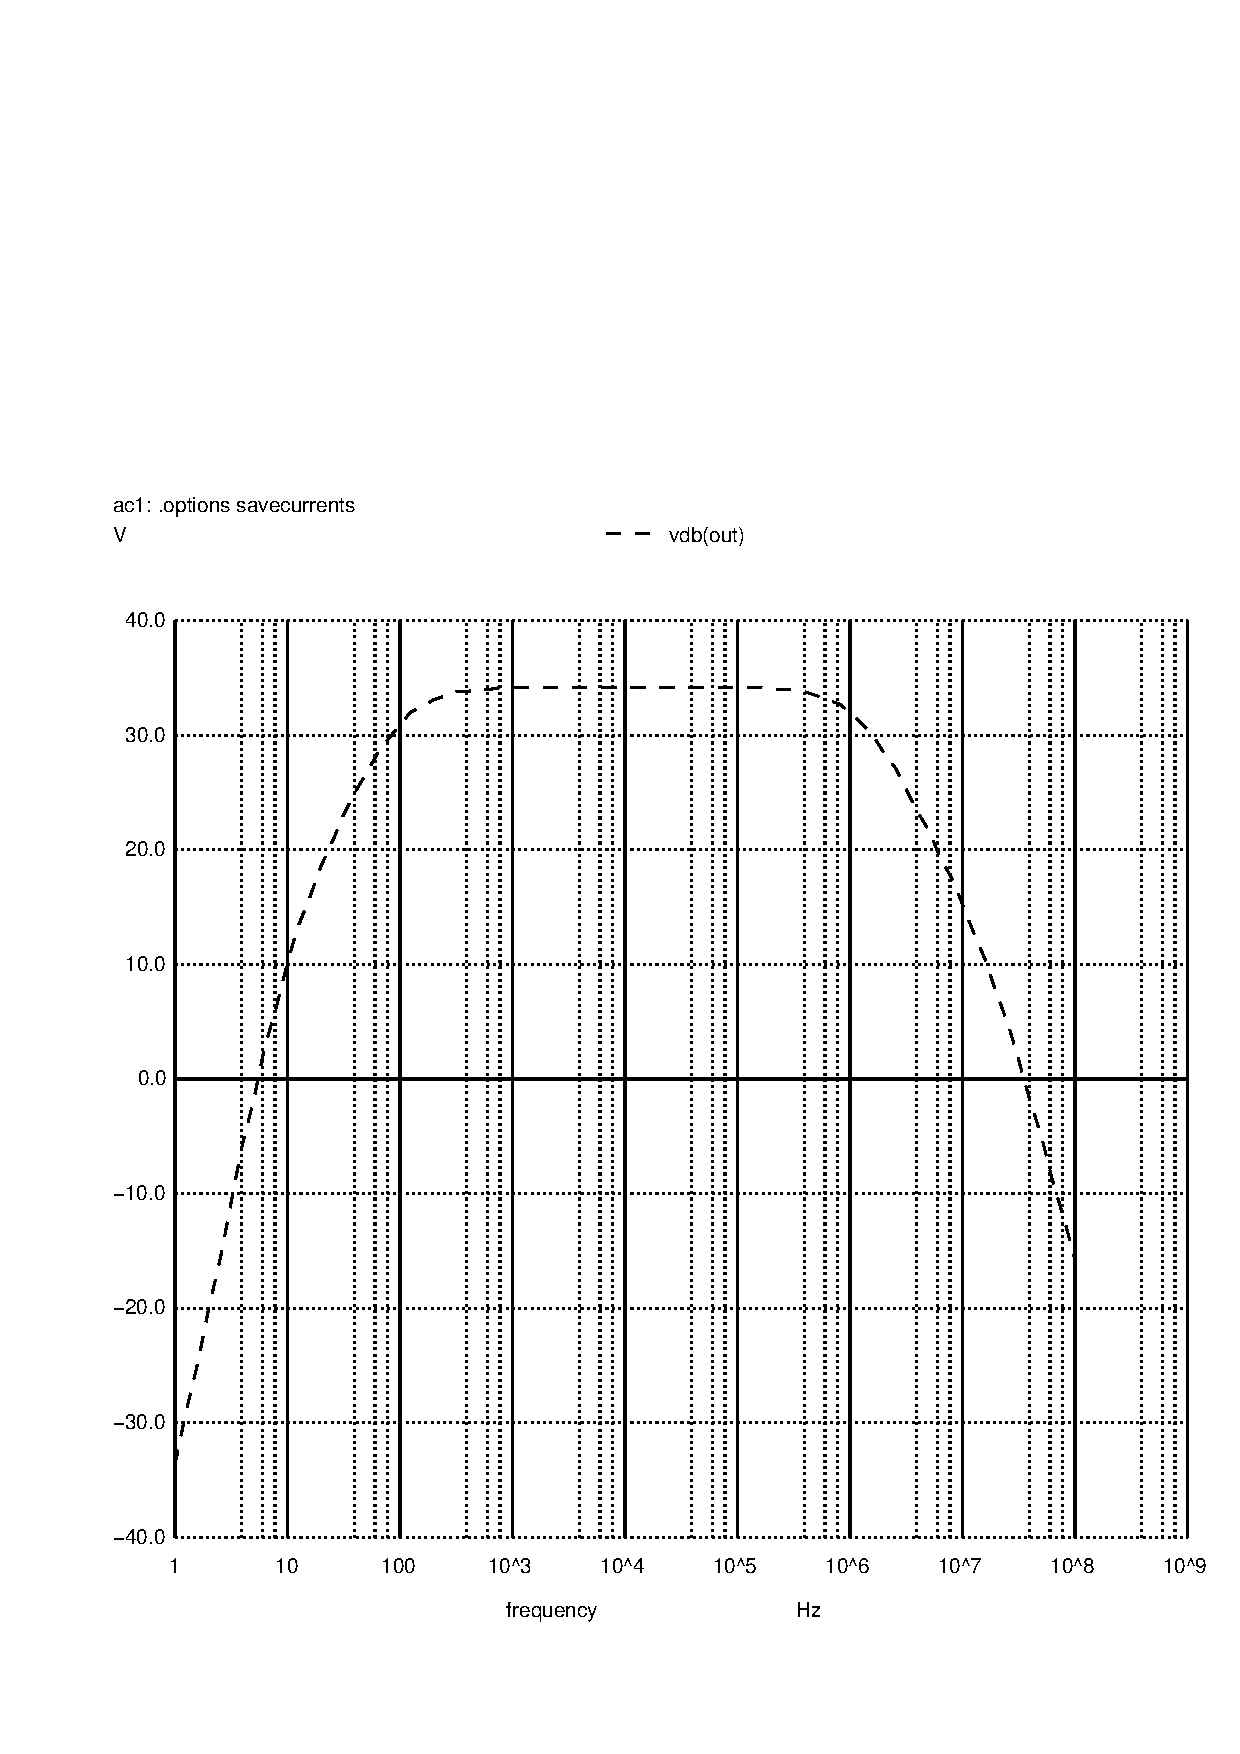
\includegraphics[width=\textwidth]{c1high.pdf}
\caption{High $C_in$}
\label{highcin}
\end{subfigure}
\begin{subfigure}{0.3\textwidth}
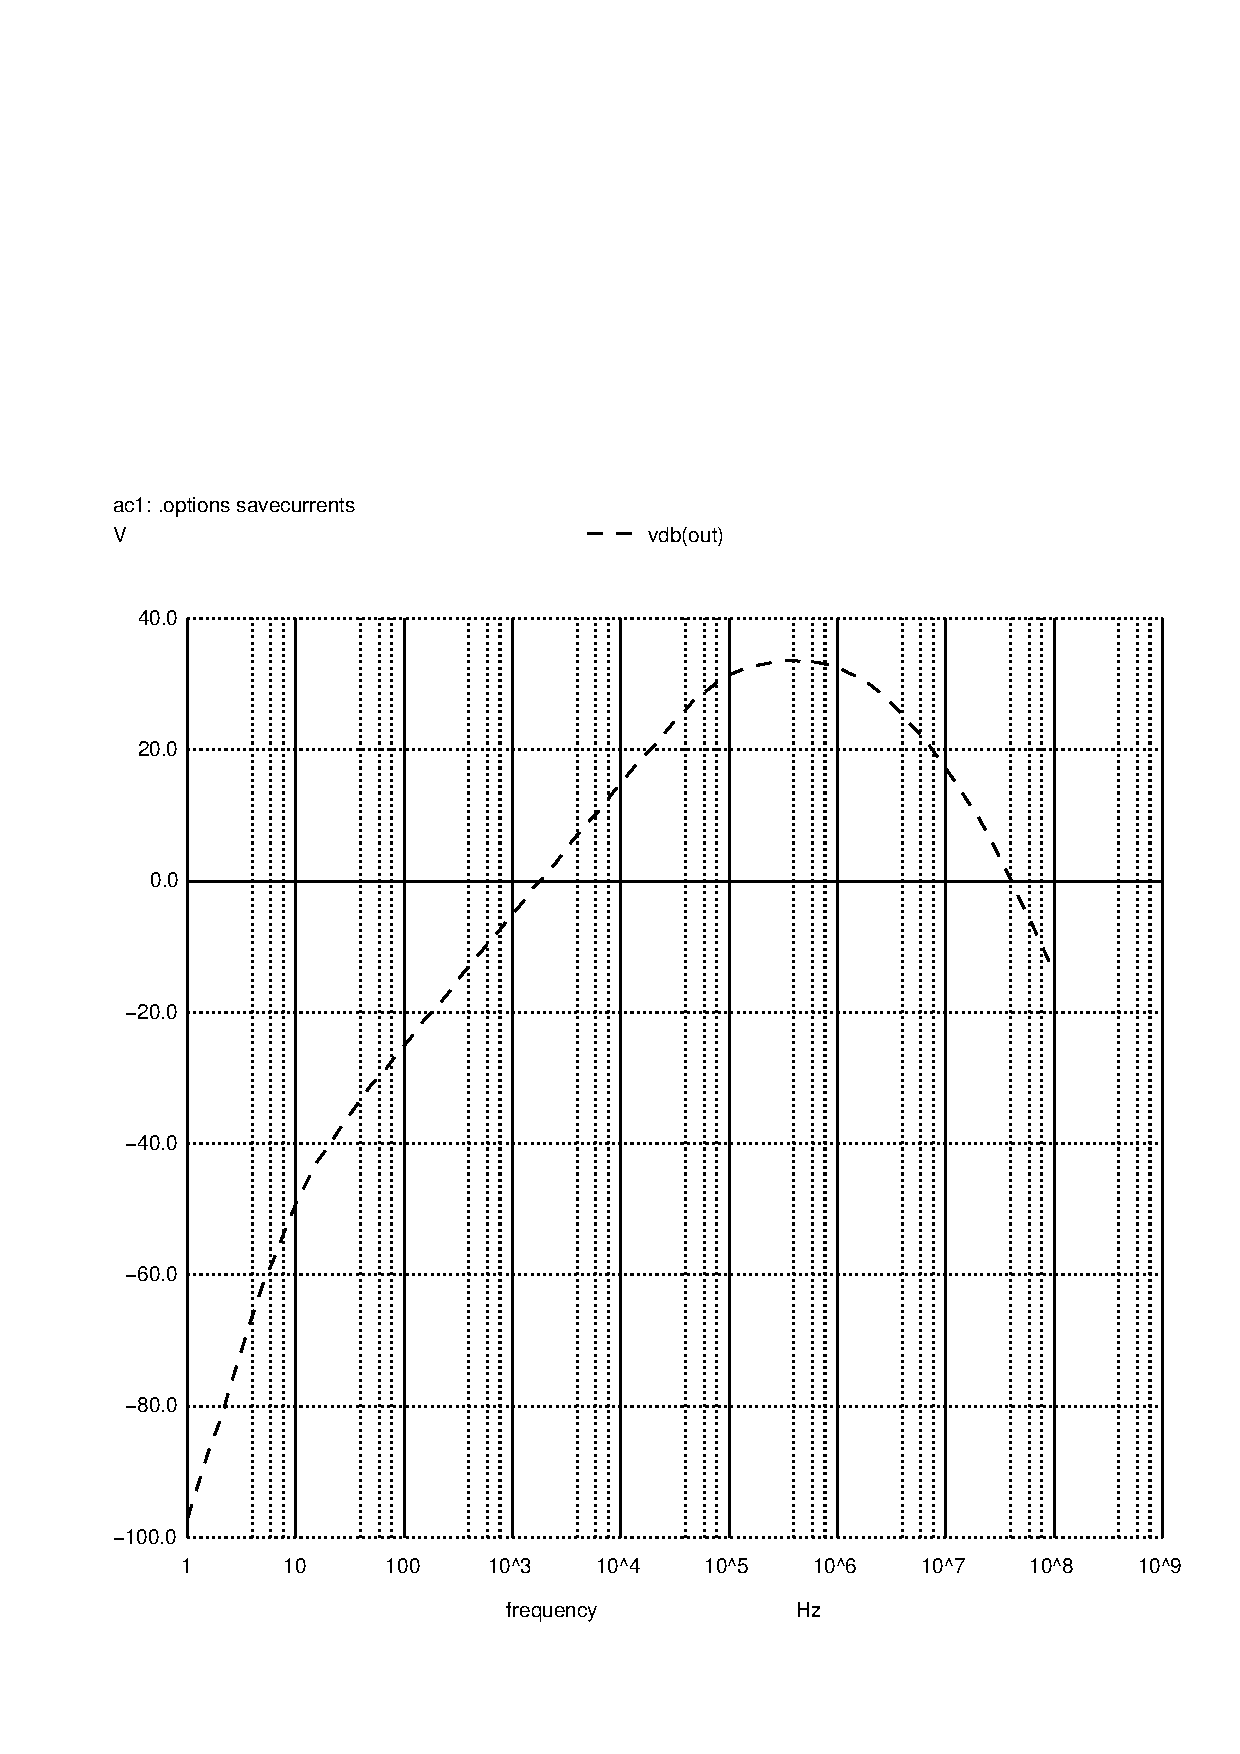
\includegraphics[width=\textwidth]{c1low.pdf}
\caption{Low $C_in$}
\label{lowcin}
\end{subfigure}
\caption{$C_in$ influence}
\end{figure}

As expected, the increase of the capacitance pushes the cutoff frequency to the left,
without changing the higher cut-off frequency, which leads to a larger bandwidth. \par
As discussed previously, as $\omega$ tends to 0, the impedance Z($C_{in}$) will tend to infinite, so this
capacitor prevents the transistor from entering on either the saturation or cut-off regions, by blocking the DC component of the AUDIO IN source. This helps mantaining the Operating Point of the transistor, so that it can operate at lower frequencies, as the value of $C_{in}$ increases.

\subsection{Bypass Capacitor}

In our Amplifier circuit there is only one bypass capacitor ($C_E$).\par 
Below, is shown 2 different graphs of the frequency response analysis, just by changing the parameter $C_E$.

\begin{figure}[H] 
\centering
\begin{subfigure}{0.4\textwidth}
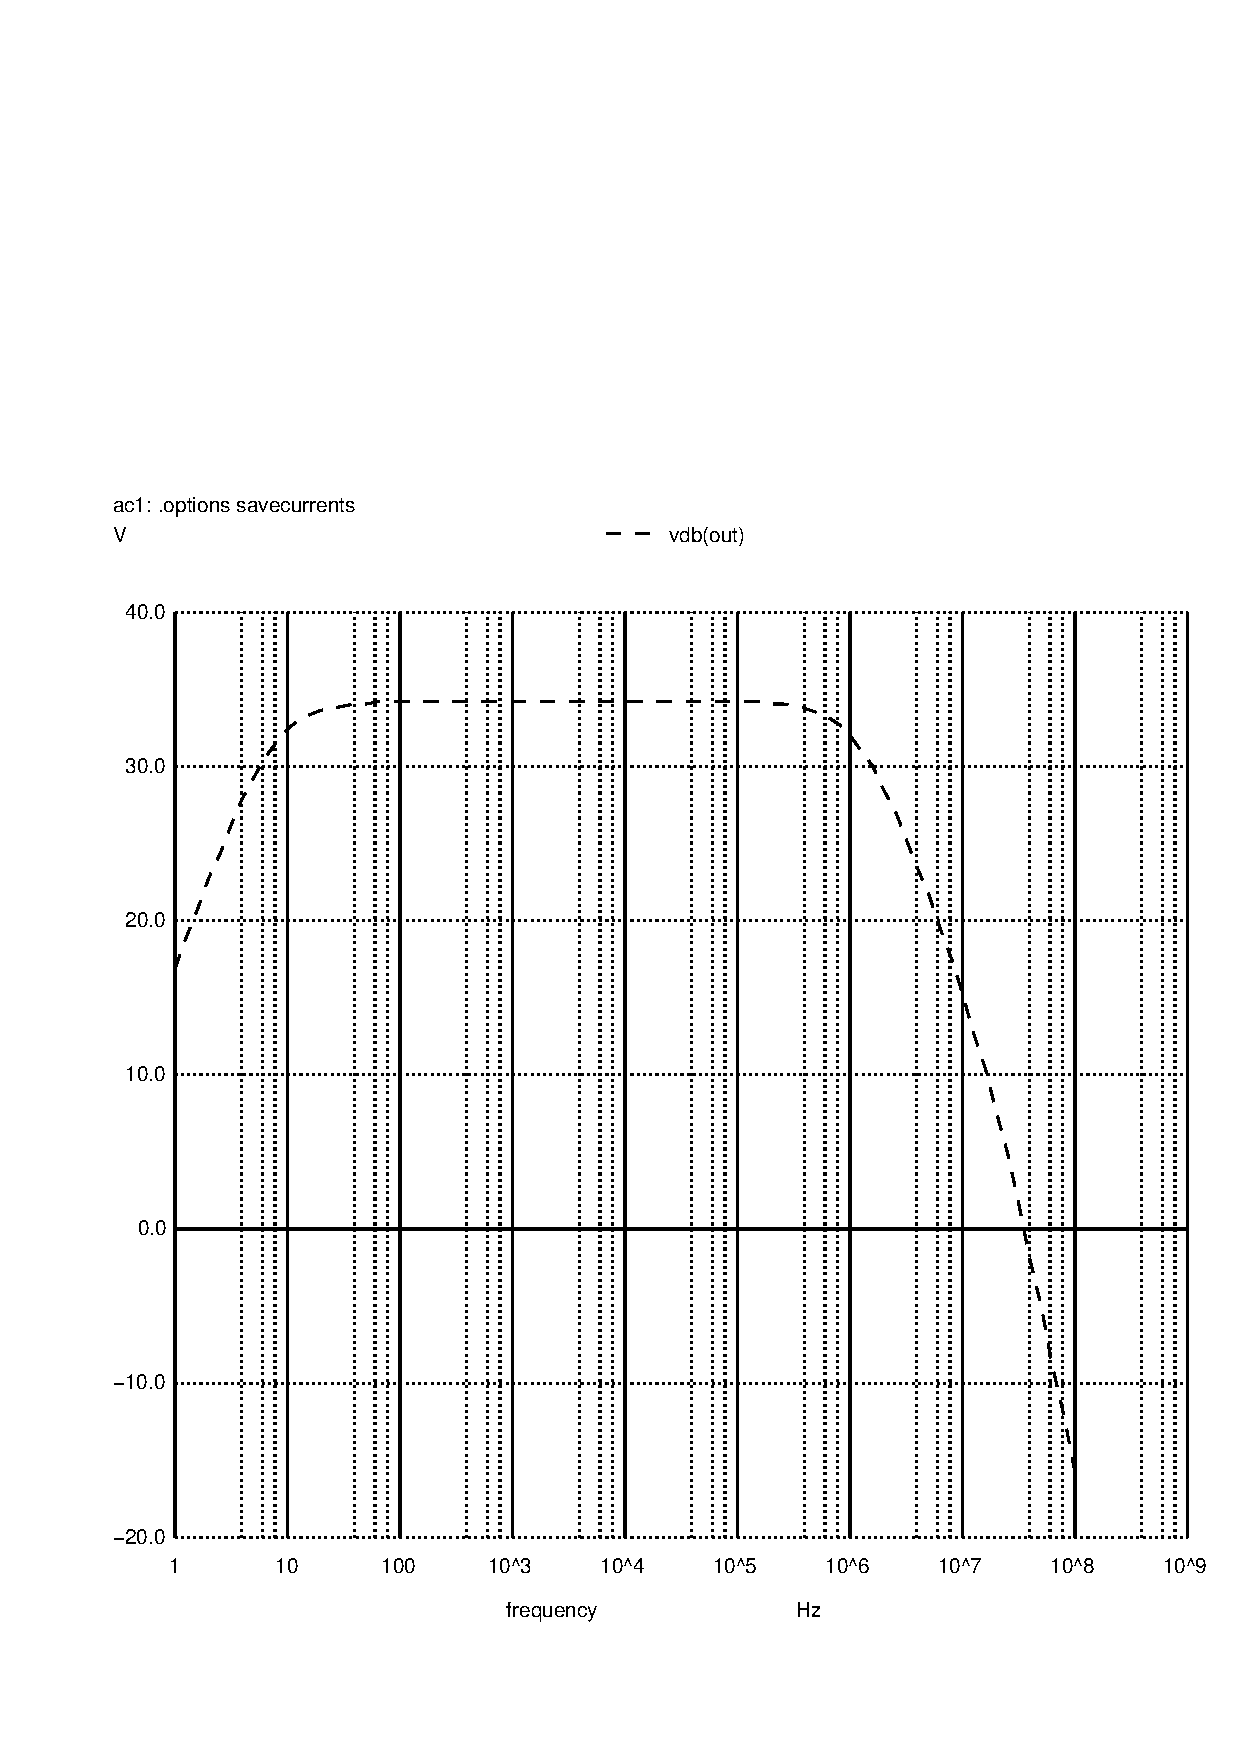
\includegraphics[width=\textwidth]{c2high.pdf}
\caption{High $C_E$}
\label{highce}
\end{subfigure}
\begin{subfigure}{0.3\textwidth}
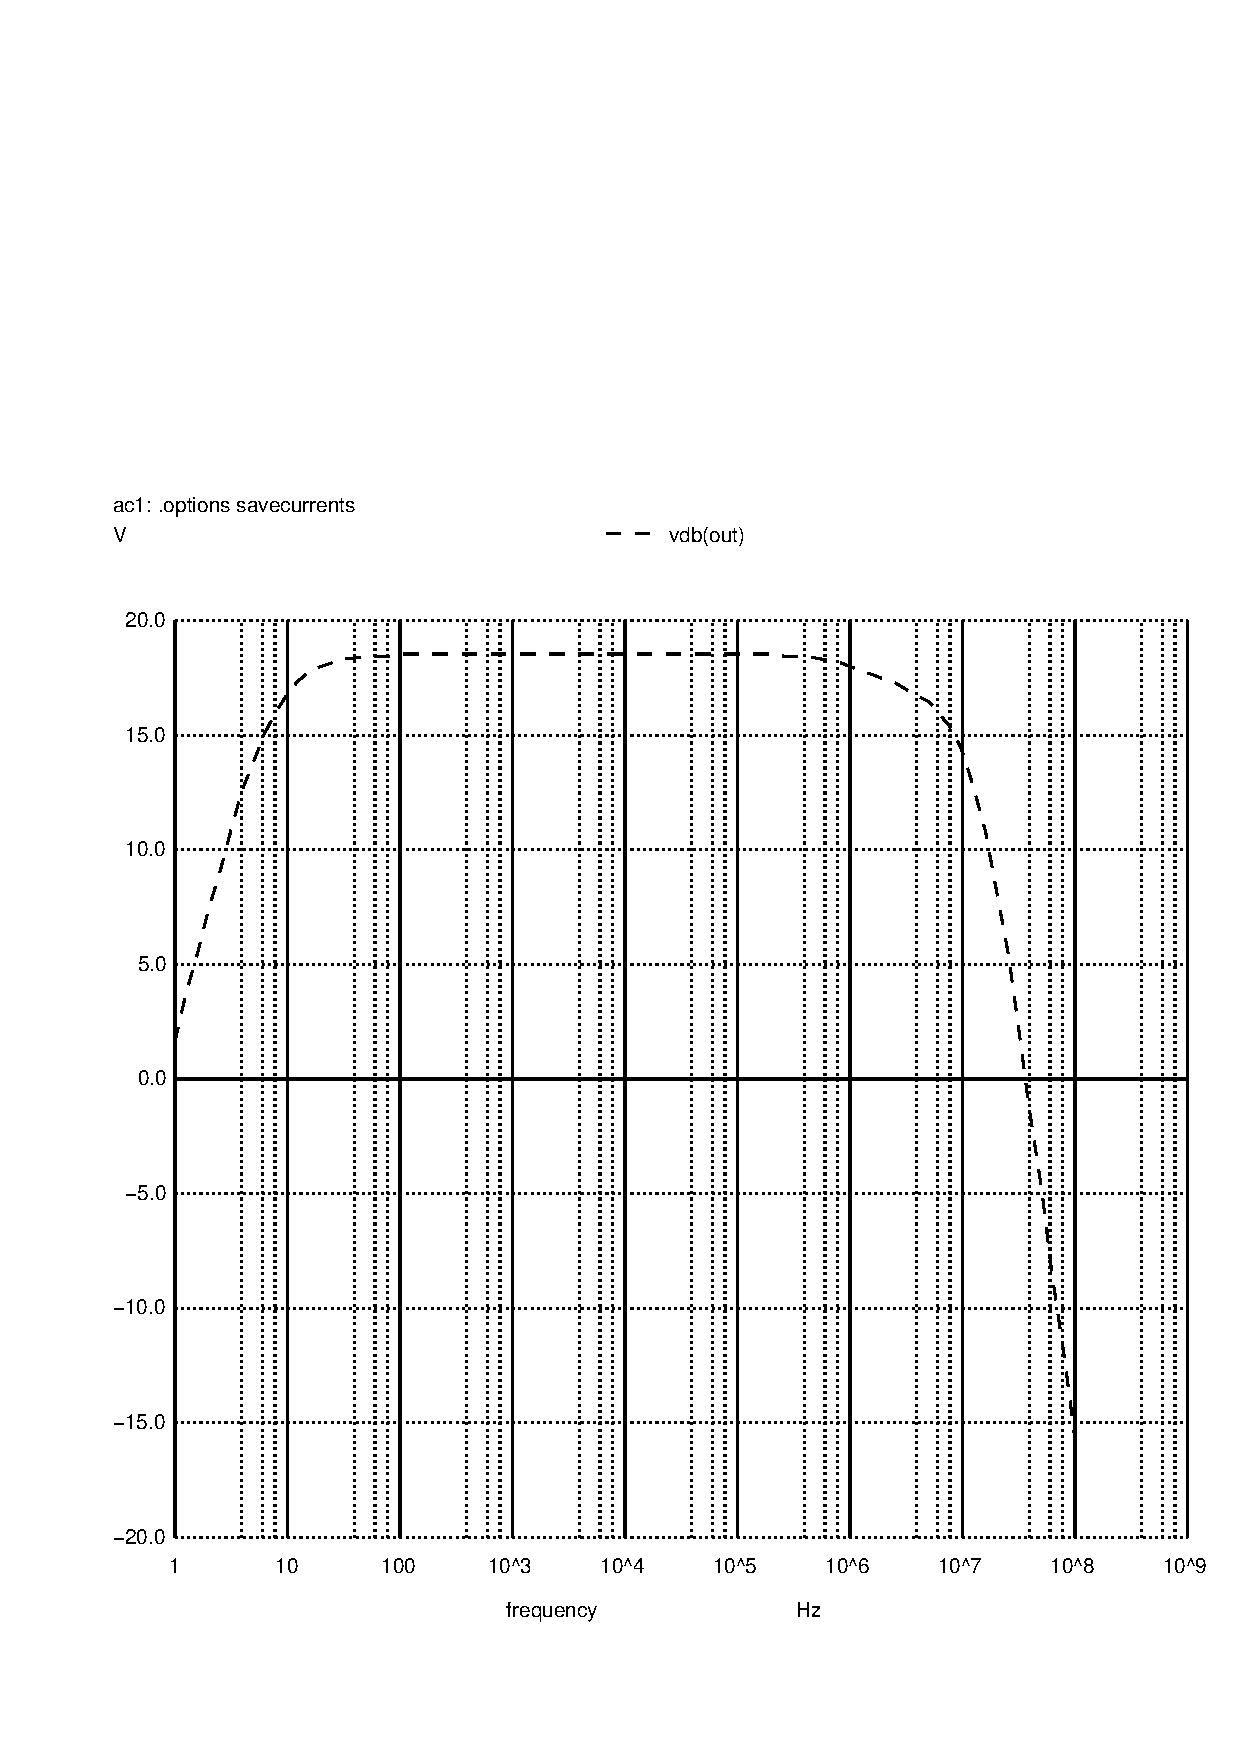
\includegraphics[width=\textwidth]{c2low.pdf}
\caption{Low $C_E$}
\label{lowce}
\end{subfigure}
\caption{$C_E$ influence}
\end{figure}

As expected, by placing the bypass capacitor in parallel with $R_E$ , this resistor becomes a short circuit for medium and high frequencies (because the capacitor impedance is 1/(j$\omega$C) and $\omega$ = 2$\pi$f). The amplifier’s first stage gain is inversely dependent on this resistance, being that the bypass capacitor plays a very important role in maximazing the gain for medium and high frequencies.

\subsection{$R_c$}

In this subsection we will analyse the importance of $R_C$ on the total Gain of the circuit.
We also present assymptotical situations in order to fully understand that behaviour.

The next graphs represent the $R_C$ influence.

\begin{figure}[H] 
\centering
\begin{subfigure}{0.4\textwidth}
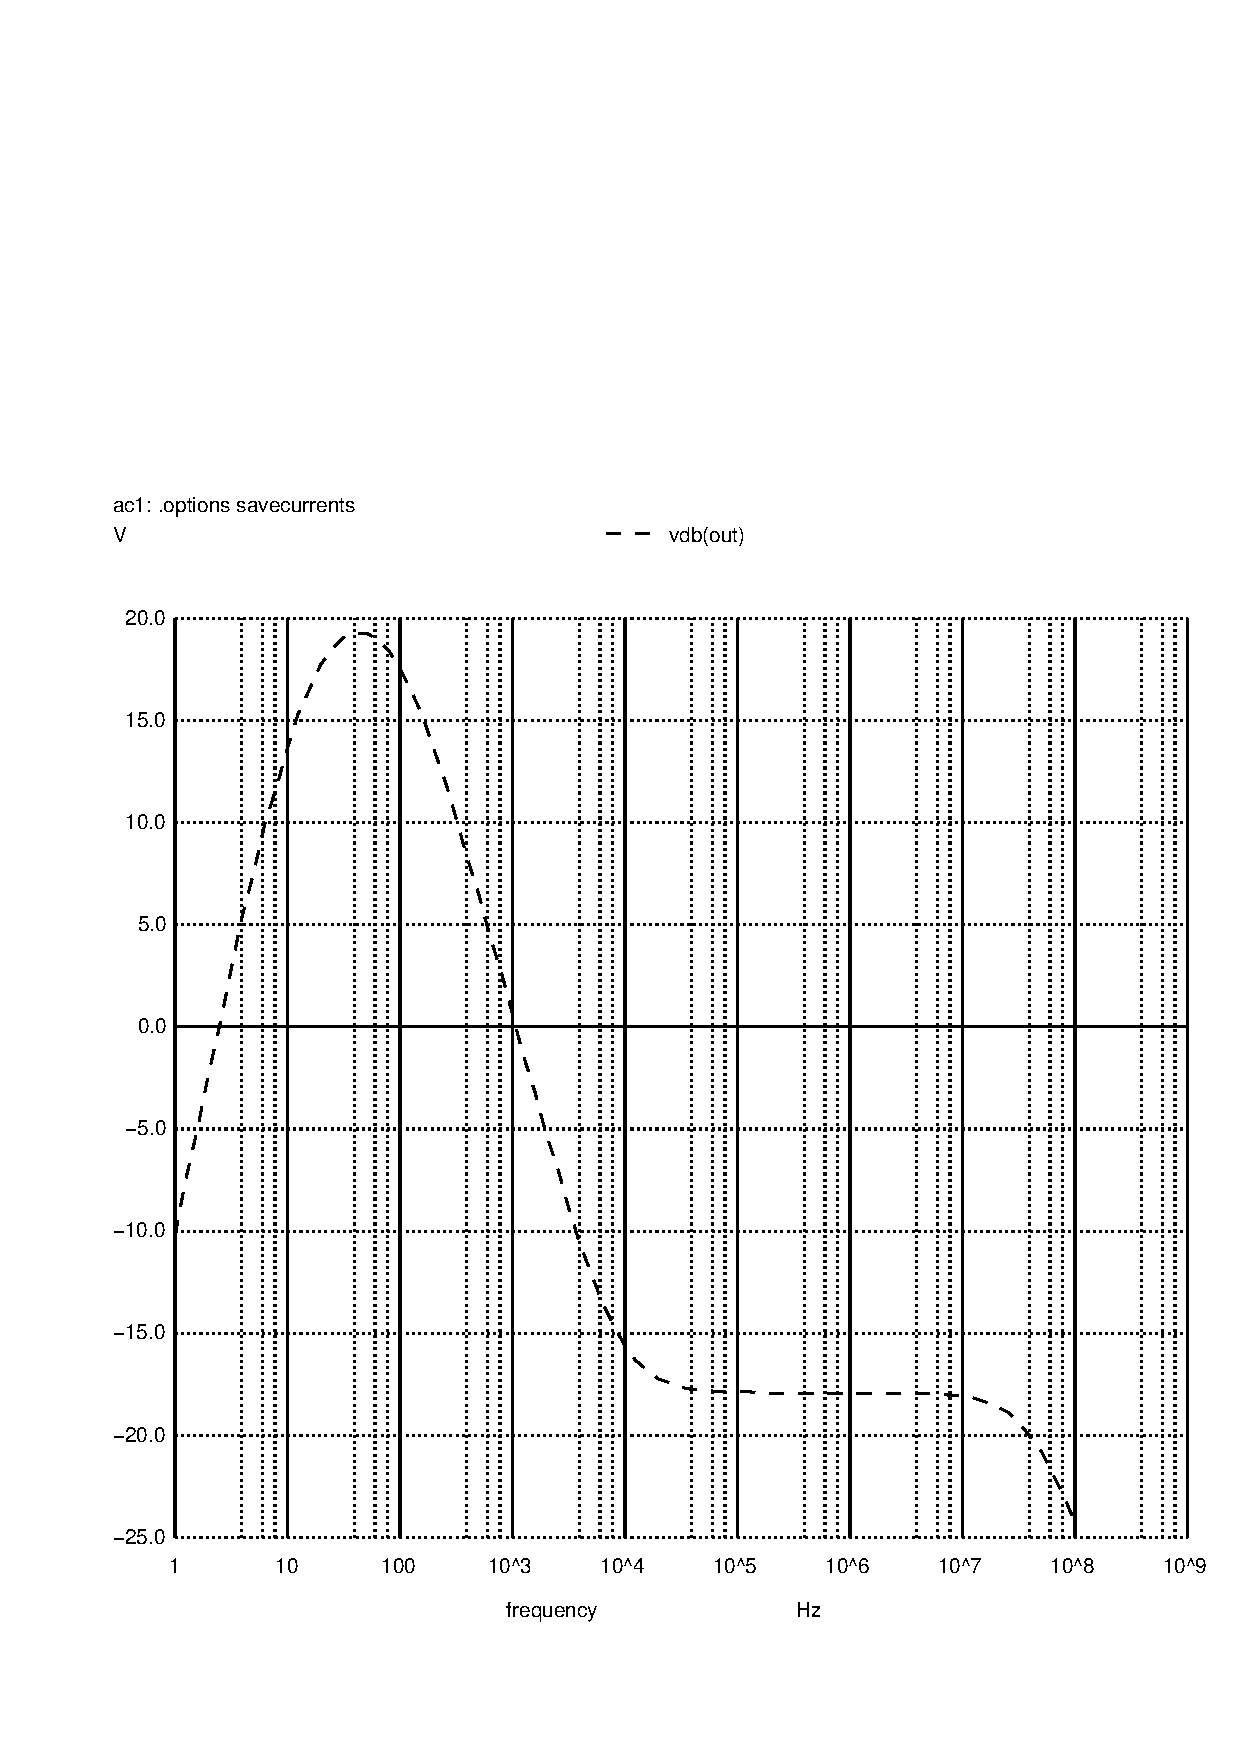
\includegraphics[width=\textwidth]{rchigh.pdf}
\caption{High $R_C$}
\label{highrc}
\end{subfigure}
\begin{subfigure}{0.3\textwidth}
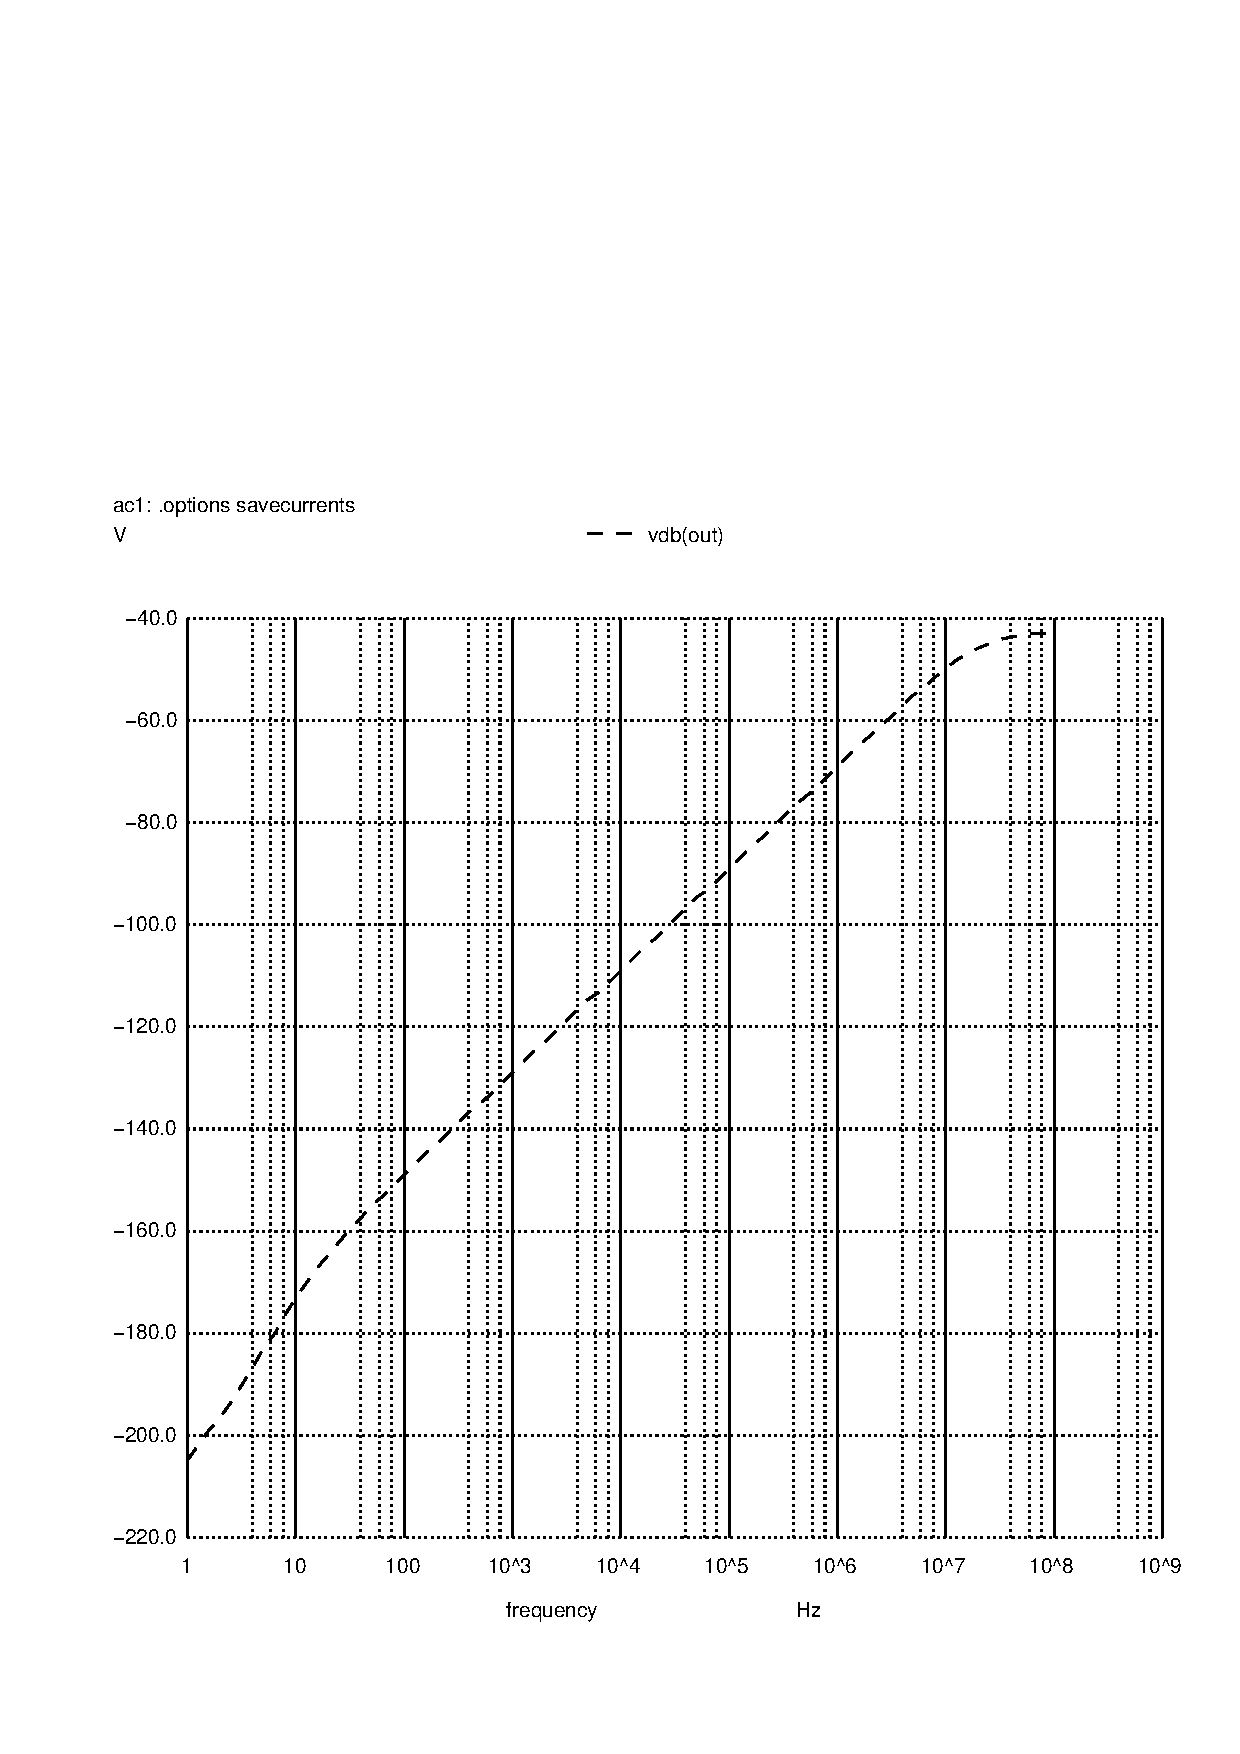
\includegraphics[width=\textwidth]{rclow.pdf}
\caption{Low $R_C$}
\label{lowrc}
\end{subfigure}
\caption{$R_C$ influence}
\end{figure}

Analysing the graphs, we can conclude that the gain increases with $R_C$ and also antecipates the passband.
This behaviour was already expected, because as described previous in the theorectical analysis of the gain, $R_C$ is proportional to the gain.
It is also important, in order to guarantee a high compatibility with AUDIO IN and to the speakers itself, to simulate the input and output impedances of the circuit. 
A good compatibility is ensured with a very high input impedance ($Z_{in}$) and a very low output impedance ($Z_{out}$). \par 
The following tables show the simulation results obtained of $Z_{in}$ and $Z_{out}$ respectively.

\begin{table}[H] \centering
\begin{tabular}{|
>{\columncolor[HTML]{FFCC67}}l |c|}
\hline
\multicolumn{2}{|l|}{\cellcolor[HTML]{EABD8B}Name - Value} \\ \hline
Zin & 999.002 + -7.3282 j\\ \hline

\end{tabular}
\caption{Results for the input impedance}
\end{table}

\begin{table}[H] \centering
\begin{tabular}{|
>{\columncolor[HTML]{FFCC67}}l |c|}
\hline
\multicolumn{2}{|l|}{\cellcolor[HTML]{EABD8B}Name - Value} \\ \hline
\input{../sim/op_ZO_TAB}
\end{tabular}
\caption{Results for the output impedance}
\end{table}

As said theoretically, the load's impedance is equal to 8$\Omega$ . The value of $Z_{out}$ should be lower than this value. \par
Given that the output value of the simulation is higher, this is going to compromise the value of the merit.

\subsection{Comparison}

Now that we have established the concepts theoretically and shown the simulation results, we are going to do a comparison between the two approaches (theoretical and simulation) with the chosen values for the constants. \par
The next graphs show the theoretical and simulation graphs of the gain respectively:

\begin{figure}[H] 
\centering
\begin{subfigure}{0.4\textwidth}
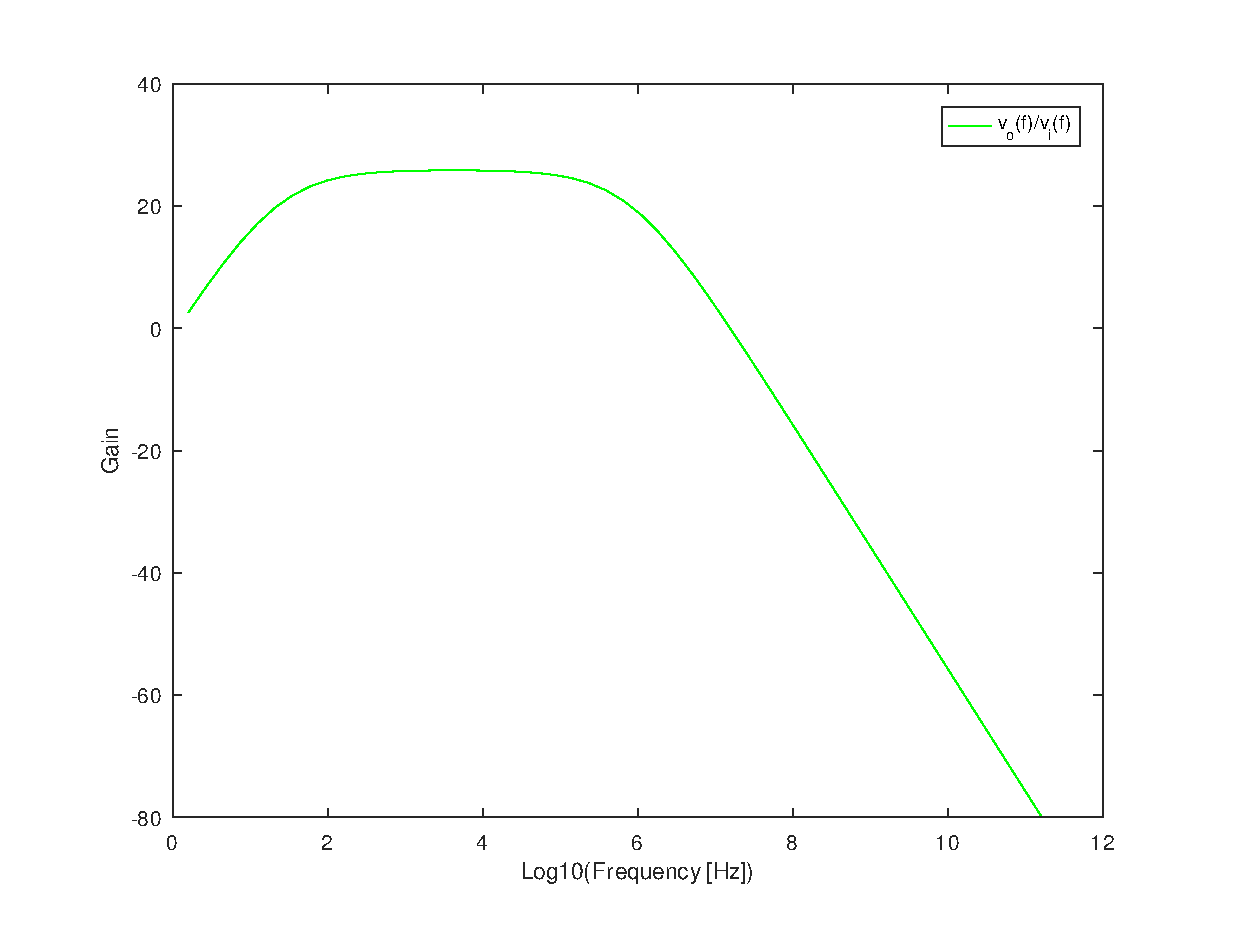
\includegraphics[width=\textwidth]{Gain.eps}
\caption{Octave}
\label{ffirst}
\end{subfigure}
\begin{subfigure}{0.3\textwidth}
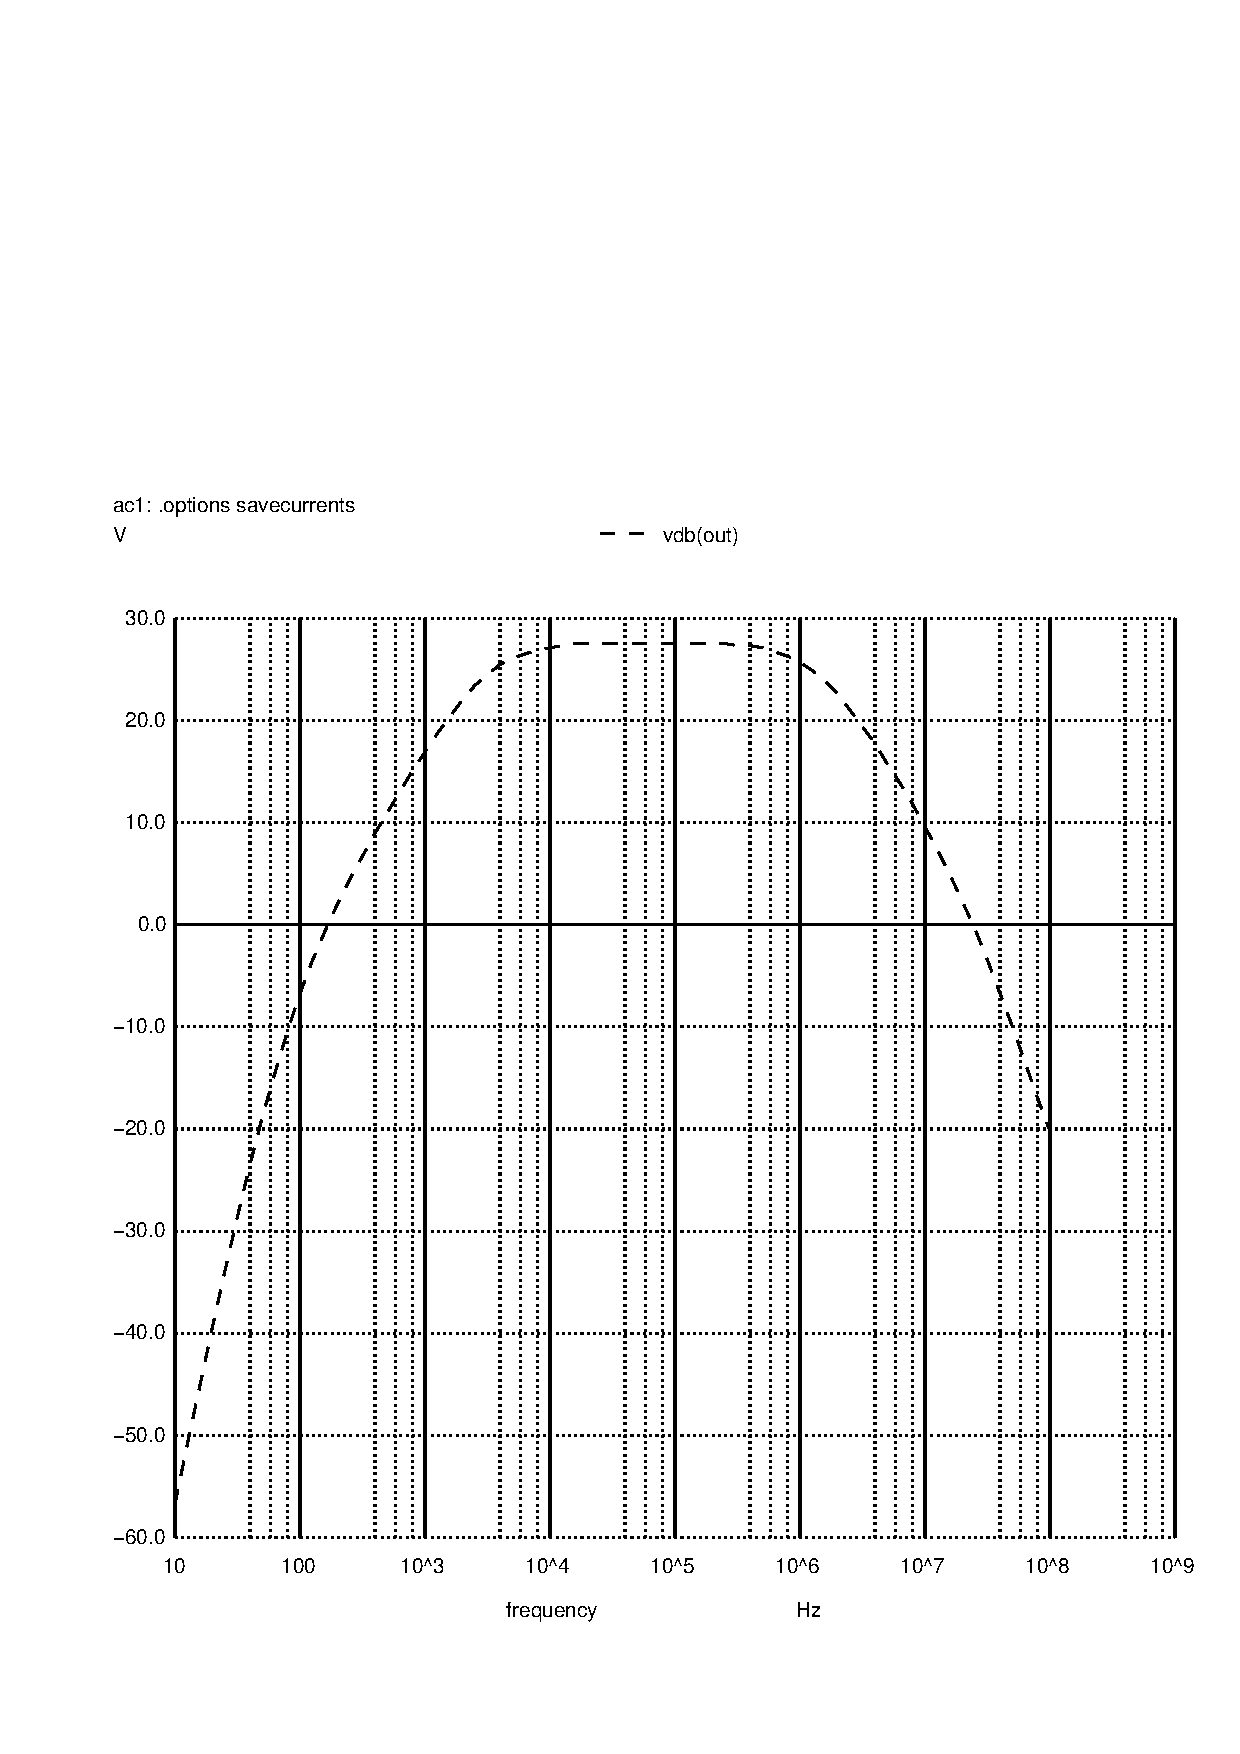
\includegraphics[width=\textwidth]{vo2f.pdf}
\caption{NgSpice}
\label{fsecond}
\end{subfigure}
\caption{Output Voltage}
\end{figure}

The comparison of the shape can only be done on the left side of the graph, because we don’t have the theoretical higher cut-off frequency, and therefore there’s no point in plotting the theoretical gain any further than 1e6 Hz. We also should be aware that the theorectical analysis either considers the capacitors open-circuited or short-circuited (this approximation is made when the value of $R_E$ is $R_E$ or 0 in Table 1, respectively).\par 
In the Octave graph we used the medium-value plot, that represents the medium between the circuit when the capacitors are open-circuit and when they are short-circuit, that is consider to be a rough approximation of the real gain. This approach doesn't guarantee a specific value for the gain, however it gives us a region of acceptable gains. In the other hand, as expected, the graph that describes the simulation gain obtained is satisfyingly in this region.
The overall shape of the graphs is similar. As it was said previously, whe while using the dominant pole aproximation can't determine what happens to the gain below the lower cutoff frequency and above the higher cutoff frquency. Subsequently, the shape of the gain graph in this regions isn't as accurate as it is below this two frequencies .\par

The next tables represent both the theoretically and the simulation results, respectivelly.

\begin{table}[H]
    \begin{minipage}{.5\linewidth}
      \centering
        \begin{tabular}{|
		>{\columncolor[HTML]{FFCC67}}l |c|}
		\hline
		\multicolumn{2}{|l|}{\cellcolor[HTML]{EABD8B}Name - Value} \\ \hline
		Zin & 999.002 + -7.3282 j\\ \hline

	\end{tabular}
      \caption{Octave}
    \end{minipage}%
    \begin{minipage}{.5\linewidth}
      \centering
        \begin{tabular}{|
		>{\columncolor[HTML]{FFCC67}}l |c|}
		\hline
		\multicolumn{2}{|l|}{\cellcolor[HTML]{EABD8B}Name - Value} \\ \hline
		Zin & 999.002 + -7.3282 j\\ \hline

	\end{tabular}
       \caption{NGspice}
    \end{minipage} 
   \caption{$Z_in$}
\end{table}

\begin{table}[H]
    \begin{minipage}{.5\linewidth}
      \centering
        \begin{tabular}{|
		>{\columncolor[HTML]{FFCC67}}l |c|}
		\hline
		\multicolumn{2}{|l|}{\cellcolor[HTML]{EABD8B}Name - Value} \\ \hline
		Zin & 999.002 + -7.3282 j\\ \hline

	\end{tabular}
      \caption{Octave}
    \end{minipage}%
    \begin{minipage}{.5\linewidth}
      \centering
        \begin{tabular}{|
		>{\columncolor[HTML]{FFCC67}}l |c|}
		\hline
		\multicolumn{2}{|l|}{\cellcolor[HTML]{EABD8B}Name - Value} \\ \hline
		Zo & 0.0522978 + -7.23396 j\\ \hline

	\end{tabular}
       \caption{NGspice}
    \end{minipage} 
   \caption{$Z_out$}
\end{table}

\begin{table}[H]
    \begin{minipage}{.5\linewidth}
      \centering
        \begin{tabular}{|
		>{\columncolor[HTML]{FFCC67}}l |c|}
		\hline
		\multicolumn{2}{|l|}{\cellcolor[HTML]{EABD8B}Name - Value} \\ \hline
		Zin & 999.002 + -7.3282 j\\ \hline

	\end{tabular}
      \caption{Octave}
    \end{minipage}%
    \begin{minipage}{.5\linewidth}
      \centering
        \begin{tabular}{|
		>{\columncolor[HTML]{FFCC67}}l |c|}
		\hline
		\multicolumn{2}{|l|}{\cellcolor[HTML]{EABD8B}Name - Value} \\ \hline
		Zin & 999.002 + -7.3282 j\\ \hline

	\end{tabular}
       \caption{NGspice}
    \end{minipage} 
   \caption{$W_L$}
\end{table}

\begin{table}[H]
    \begin{minipage}{.5\linewidth}
      \centering
        \begin{tabular}{|
		>{\columncolor[HTML]{FFCC67}}l |c|}
		\hline
		\multicolumn{2}{|l|}{\cellcolor[HTML]{EABD8B}Name - Value} \\ \hline
		Zin & 999.002 + -7.3282 j\\ \hline

	\end{tabular}
      \caption{Octave}
    \end{minipage}%
    \begin{minipage}{.5\linewidth}
      \centering
        \begin{tabular}{|
		>{\columncolor[HTML]{FFCC67}}l |c|}
		\hline
		\multicolumn{2}{|l|}{\cellcolor[HTML]{EABD8B}Name - Value} \\ \hline
		Zin & 999.002 + -7.3282 j\\ \hline

	\end{tabular}
       \caption{NGspice}
    \end{minipage} 
   \caption{$W_H$}
\end{table}

\begin{table}[H]
    \begin{minipage}{.5\linewidth}
      \centering
        \begin{tabular}{|
		>{\columncolor[HTML]{FFCC67}}l |c|}
		\hline
		\multicolumn{2}{|l|}{\cellcolor[HTML]{EABD8B}Name - Value} \\ \hline
		Zin & 999.002 + -7.3282 j\\ \hline

	\end{tabular}
      \caption{Octave}
    \end{minipage}%
    \begin{minipage}{.5\linewidth}
      \centering
        \begin{tabular}{|
		>{\columncolor[HTML]{FFCC67}}l |c|}
		\hline
		\multicolumn{2}{|l|}{\cellcolor[HTML]{EABD8B}Name - Value} \\ \hline
		Zin & 999.002 + -7.3282 j\\ \hline

	\end{tabular}
       \caption{NGspice}
    \end{minipage} 
   \caption{$A_v$}
\end{table}

With the values side by side, in a more detailed analysis, of $Z_{in}$, $Z_{out}$ ,$A_V$,$\omega _{CO_H}$ and $\omega _{CO_L}$ despite the obvious differences, the comparison is satisfatory. When comparing the order of magnitude they are within reasonable intervals of similarity. In fact, the lower cut-off frequencies are really similar, especially when they are plotted in a logscale graph.

\subsection{Merit Results}
\label{merit}

From the results obtained through the Ngspice simulation and considering we used the data shown in table 1, we can compute the merit using the formula given in the lab assignment, represented in the Introduction.

The values of cost and merit are represented in the next table:

\begin{table}[H] \centering
\begin{tabular}{|
>{\columncolor[HTML]{FFCC67}}l |c|}
\hline
\multicolumn{2}{|l|}{\cellcolor[HTML]{EABD8B}Name - Value} \\ \hline
Cost & 2619.6\\ \hline
merit & 1262.83\\ \hline

\end{tabular}
\caption{Cost and Merit}
\end{table}

To obtain the best values for the circuit, we've used the matlab simulink to optimize them for the best merit.

